\subsection{UC-14}
\label{subsec:UC-14}

\begin{figure}[H]
    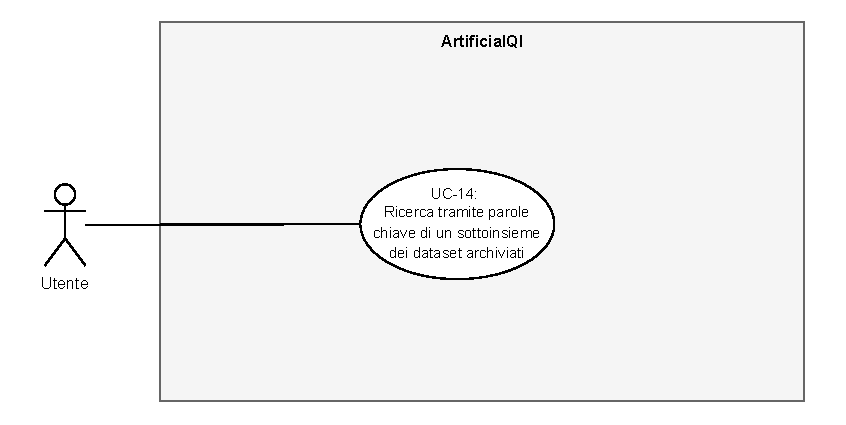
\includegraphics{Sezioni/UseCase/Immagini/UC-14.pdf}
    \caption{Diagramma UC-14.}
\end{figure}

\begin{usecase}{UC-14}{Caricamento di un dataset precedentemente archiviato come dataset corrente}

    \req{\hyperref[item:RU-4]{RU-4}} 

    \pre{
        \item Il sistema è attivo e funzionante
        \item Esiste almeno un dataset archiviato nel sistema
    }

    \post{
        \item Il dataset da caricare diventa il dataset corrente
    }
    
    \actor{Utente}

    \subactors{}

    \trigger{L'utente deve caricare un dataset tra quelli archiviati nel sistema}
    
    \inc{}

    \base{}

    \scenario{
        \item L'utente richiede di caricare un dataset archiviato nel sistema
        \item L'utente seleziona il nome del dataset tra quelli archiviati
        \item Il dataset scelto viene caricato come dataset corrente
    }

    \subscenario{
        \item[3.1] \textbf{Il dataset corrente non è vuoto e non possiede una versione aggiornata archiviata}
        \begin{itemize}
            \item[a.] \hyperref[subsec:UC-15]{UC-15}
        \end{itemize}
    }
\end{usecase}